\chapter{Μετάδοση Γνώσης}%
\label{chapter:tl}
\section{Εισαγωγή}
Ο όρος της μετάδοσης γνώσης(Transfer Learning) χρησιμοποιείται σε όλο το φάσμα της τεχνητής νοημοσύνης ως η μεταφορά παραμέτρων ενός ήδη εκπαιδευμένου συστήματος σε ένα άλλο. Στο παρόν κεφάλαιο θα αναλυθεί η μετάδοση γνώσης σε αλγορίθμους εντοπισμού αντικειμένων· βέβαια για την καλύτερη ανάλυση αρχικά θα πρέπει να δοθούν κάποιοι ορισμοί και να ερμηνευτεί με ακρίβεια ο όρος. Έπειτα, θα αναλυθούν οι τρόποι μετάδοσης γνώσης όπως φαίνονται στο Σχήμα \ref{fig:TL_categories}. Στο τέλος παρουσιάζεται το πείραμα αυτής της εργασίας για τα δίκτυα εντοπισμού αντικειμένων.

\begin{figure}
    \centering
    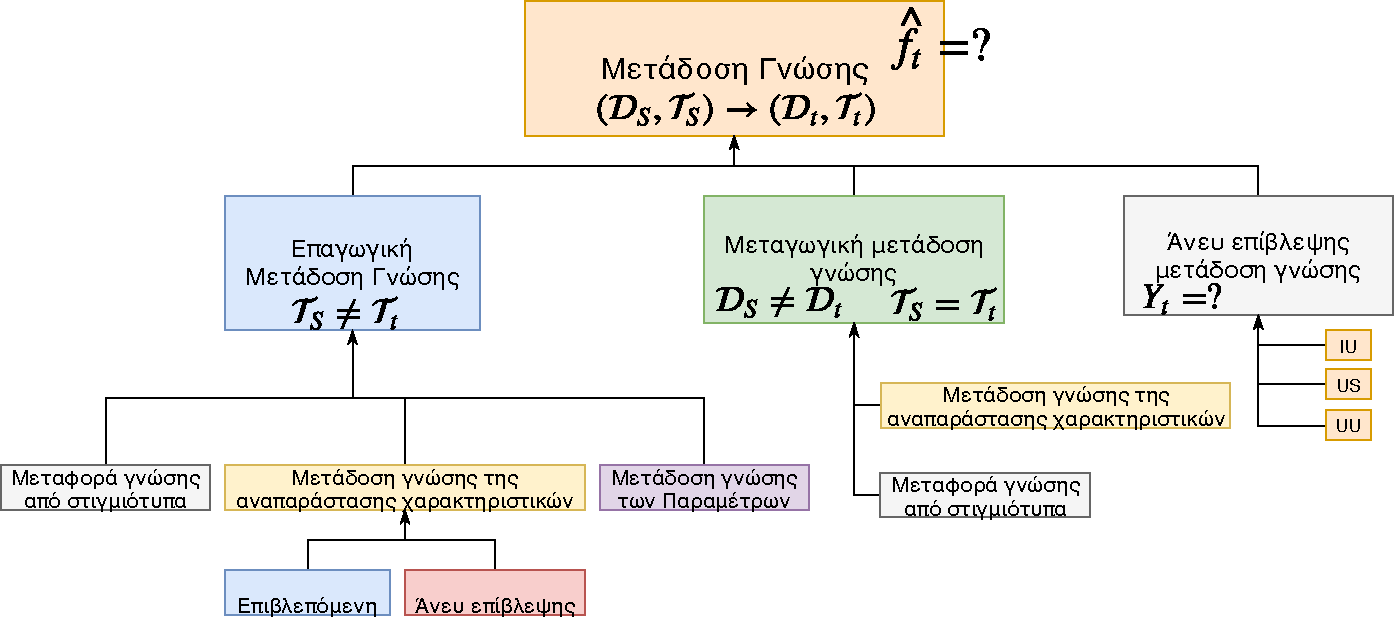
\includegraphics[width = 0.8\textwidth]{figures/transferLearning/TL_categorisation.pdf}
    \caption[Οι κατηγορίες της μετάδοσης γνώσης]{Η κατηγοριοποίηση των διάφορων ειδών μετάδοσης γνώσης. Στο πρώτο (πάνω) επίπεδο φαίνεται η φορά πληροφορίας και ο τελικός σκοπός όλης της μετάδοσης γνώσης. Στο δεύτερο επίπεδο φαίνεται οι σχέσεις μεταξύ του αρχικού και τελικού προβλήματος στα τρία σενάρια μετάδοση γνώσης. Στο τελευταίο επίπεδο παρουσιάζονται οι διάφορες προσεγγίσεις σε κάθε μία από τις κατηγορίες. Όλα αυτά αναλύονται με λεπτομέρεια στο παρόν κεφάλαιο.}
    \label{fig:TL_categories}
\end{figure}

\section{Πρόβλημα}
Το πρόβλημα που αντιμετωπίζεται στα νευρωνικά δίκτυα έγκειται στο θεώρημα \textit{no free lunch} \cite{37}. H
θεωρία της μηχανικής μάθησης υποστηρίζει ότι οι αλγόριθμοι μηχανικής μάθησης μπορούν να γενικευτούν σε ένα πεπερασμένο σύνολο από παραδείγματα. Ωστόσο, αυτό δείχνει να αντιτίθεται σε κάποιες βασικές αρχές της λογικής. Η επαγωγή γενικών κανόνων από κάποιο πεπερασμένο σύνολο παραδειγμάτων δεν αποτελεί λογικό εγχείρημα. Για παράδειγμα, προκειμένου να δημιουργηθεί ένας κανόνας ο οποίος να περιγράφει κάθε μέλος ενός συνόλου, θα πρέπει εκ των προτέρων να υπάρχει πληροφορία για κάθε μέλος αυτού του συνόλου.

Εν μέρει η μηχανική μάθηση προσπερνά αυτό το πρόβλημα προσφέροντας μόνο πιθανοτικούς κανόνες, αντί για ακριβείς κανόνες που αποτελούν μέλη της μαθηματικής λογικής. Η μηχανική μάθηση υπόσχεται να βρει κανόνες οι οποίοι είναι πιθανοτικά έγκυροι για τα περισσότερα μέλη κάποιου συνόλου. Δυστυχώς, ακόμη και αυτό δεν μπορεί να επιλύσει το όλο πρόβλημα. Σύμφωνα με το θεώρημα \textit{no free lunch}, ο μέσος όρος σφάλματος σε όλες τις πιθανές κατανομές σημείων εισόδου, για κάθε αλγόριθμο κατηγοριοποίησης είναι ο ίδιος με την κατηγοριοποίηση σημείων τα οποία δεν έχουν παρατηρηθεί εκ των προτέρων.

Αν $ \mathbb{K} $ είναι το σύνολο όλων των πιθανών κατανομών και $ \kappa_i, \kappa_j \in \mathbb{K}$ δύο κατανομές στις οποίες έχουν εκπαιδευτεί
οι αλγόριθμοι $a_i, a_j$ αντίστοιχα. Τότε για συνάρτηση σφάλματος $e(a,\kappa)$ αλγορίθμου $a$ σε κάποια κατανομή $\kappa \in \mathbb{K}$, ισχύει:
$$ \EX_{\kappa \in \mathbb{K}-\kappa_i}\left[ e(a_i, \kappa) \right] = \EX_{\kappa \in \mathbb{K}-\kappa_j}\left[ e(a_j, \kappa) \right], \forall i,j
$$ 

Δηλαδή, κανένας αλγόριθμος δεν είναι καλύτερος στην επίλυση καινούριων προβλημάτων από ότι ένας άλλος. Ευτυχώς,
αυτό συμβαίνει μόνο όταν λαμβάνονται υπόψη όλες οι πιθανές κατανομές. Στον πραγματικό κόσμο μπορούν να γίνουν κάποιες
υποθέσεις για τους τύπους κατανομών που αντιμετωπίζονται και μπορεί να γίνει ο ισχυρισμός ότι αυτές ανήκουν σε συγκεκριμένες πολλαπλότητες.
Παρόλα αυτά, απαιτείται το δίκτυο εντοπισμού να είναι πραγματικού χρόνου και περιορισμένης μνήμης. Έτσι, δεν μπορεί 
να συμπεριλάβει χαρακτηριστικά για να αφομοιώσει όλη την εμπειρία που απαιτείται για να εντοπίζει εκ των προτέρων κάθε αντικείμενο.

\section{Μία ιδέα για τη μετάδοση γνώσης \cite{38}}
Η μετάδοση γνώσης είναι μία ανθρώπινη διαδικασία η οποία έχει μελετηθεί πολύ στην
φιλοσοφία, στην εκπαίδευση και στην εκπαιδευτική ψυχολογία \cite{39}. Στην εκπαίδευση, η μετάδοση
γνώσης αναφέρεται ως:
"Προηγουμένως μαθημένες γνώσεις ή ικανότητες οι οποίες επηρεάζουν τον τρόπο με τον οποίο
μία καινούρια γνώση ή ικανότητα μαθαίνεται και χειρίζεται. Η μετάδοση θεωρείται ως θετική
αν η απόκτηση και η επίδοση στην χρήση της καινούριας γνώσης διευκολύνθηκε και ως αρνητική
αν εμποδίστηκε."(μετάφραση από: \cite{76})

Όταν η τεχνική μετάδοσης γνώσης εφαρμόζεται στη μηχανική μάθηση έχει παρόμοιο σκοπό. Το κίνητρο της μηχανικής μάθησης είναι να βελτιώσει τη μάθηση σε ένα συγκεκριμένο πεδίο αποκτώντας πληροφορία από ένα παρόμοιο, αλλά διαφορετικό πεδίο. Οι παραδοσιακές τεχνικές μηχανικής μάθησης, όπως λέχθηκε λειτουργούν υπό υποθέσεις για τις κατανομές τους. Για αυτό και παλαιότερα προτεινόταν η μάθηση να αρχίζει \textit{tabula rasa}, χωρίς να ξέρει τίποτε πιο πριν ο αλγόριθμος και όλοι οι παράμετροι των δικτύων ή των αλγορίθμων να αρχίζουν από κάποια τυχαία κατανομή όπως η γκαουσιανή. Επιπλέον, υπάρχει η ανάγκη από την πλειοψηφία των τεχνικών μηχανικής μάθησης τα δεδομένα στα σύνολα της εκπαίδευσης και του ελέγχου να είναι από τον ίδιο χώρο χαρακτηριστικών (feature space).
Η τεχνική μετάδοσης γνώσης δείχνει πως αυτό δεν είναι σε κάθε περίπτωση απαραίτητο για τα νευρωνικά δίκτυα, γιατί δίνεται η δυνατότητα να συνδυαστεί προηγούμενη γνώση από μία προηγούμενη εκπαίδευση σε μία καινούρια αλλά σχετική με την προηγούμενη.

Χρησιμοποιώντας αυτή την παρατήρηση μπορεί να παρακάμψει κανείς το \textit{no free lunch theorem}, 
διότι δεν χρειάζεται ανά πάσα στιγμή να είναι δυνατός ο εντοπισμός όλων των αντικειμένων. Ο αλγόριθμος μπορεί  να ξέρει κάθε στιγμή να εντοπίζει ένα μικρό σύνολο αντικειμένων και απλά κάθε φορά να μαθαίνει τον εντοπισμό ενός καινούριου συνόλου.

\section{Ορισμός της Μετάδοσης Γνώσης \cite{40, 41}}
Πριν τη μετάβαση στον μαθηματικό ορισμό της τεχνικής μετάδοσης γνώσης θα πρέπει να ορισθούν κάποια άλλα μεγέθη
πρώτα. Οι ορισμοί αυτοί μπορούν να χρησιμοποιηθούν γενικότερα στο αντικείμενο της μηχανικής μάθησης, ωστόσο συνίσταται η χρήση τους μόνο στο αντικείμενο της μετάδοσης γνώσης.
\vspace{1ex}\\
{ \rule{1ex}{1ex} }%
\textit{Το πεδίο ορισμού(\textit{Domain}) ορίζεται ως μία δυάδα $D = (\mathcal{X},P)$. Το πρώτο μέλος της δυάδας $\mathcal{X}$ είναι ο χώρος (πολλαπλότητα) στον οποίο ανήκουν τα δείγματα-παρατηρήσεις $x$ κάποιου προβλήματος (π.χ. ο χώρος των διδιάστατων εικόνων για εικόνες μεγέθους $1024 \times 768$). Το δεύτερο μέλος της δυάδας είναι η αθροιστική συνάρτηση κατανομής $P(X)$ όπου $X = {x_1 , \cdots , x_n } \in \mathcal{X}$. }

Η εκπαίδευση, η οποία ορίζεται και παρακάτω, γίνεται πάντα σε ένα πεπερασμένο κομμάτι του πεδίου ορισμού, διότι εκτελείται από κάποιον αλγόριθμο και διαρκεί πεπερασμένο χρόνο.
\vspace{1ex}\\
{ \rule{1ex}{1ex} }%
\textit{Δοθέντος ενός πεδίου ορισμού, το υποψήφιο έργο(task) αποτελείται από την δυάδα $(\mathcal{Y}, f(.))$. Το πρώτο μέλος της δυάδας είναι ο χώρος ετικετών $\mathcal{Y}$(π.χ. τα ονόματα των κλάσεων των αντικειμένων σε μία εικόνα και ορθογώνια πάνω στην εικόνα όπου αυτά παρατηρούνται). Το δεύτερο είναι μία συνάρτηση ετικετοποίησης $ f:\mathcal{X} \rightarrow Y$. Το έργο συμβολίζεται με το γράμμα $\mathcal{T}$.}
% πορεί να χρησιμοποιηθεί για να δημιουργήσει το σετ δεδομένων το οποίο ορίζεται ως: $\left(x_i, y_i\right) = \left(x_i, f(x_i)\right)$ όπου  $ x_i \in \mathcal{X}$ και $y_i \in Y$ και συνήθως είναι πεπερασμένο.

Η συνάρτηση ετικετοποίησης "προβλέπει" πάντα ορθά την ετικέτα δοθείσας μίας εισόδου. Από πιθανοτική σκοπιά η $f(x)$ μπορεί να γραφεί ως $P(y|x)$. 
\vspace{1ex}\\
{ \rule{1ex}{1ex} }%
\textit{Το μοντέλο $M$ ορίζεται ως μία συνάρτηση $M(x;W)$, $M:\mathcal{X}\times \mathbb{W} \rightarrow Y$. Το $x$ είναι η είσοδος του μοντέλου, ενώ το $W$ είναι οι παράμετροί του. Το μοντέλο είναι δυνατόν μέσα από την εκπαίδευση (και τη ρύθμιση των παραμέτρων του) να προσεγγίσει μία συνάρτηση $f$ στο κοινό τους σύνολο ορισμού.}
\vspace{1ex}\\
{ \rule{1ex}{1ex} }%
\textit{Το πεδίο ορισμού δεδομένων ή γνωστό ως σύνολο δεδομένων ορίζεται ως $\mathcal{D}_d =\{(x_1, y_1), \dotsc, (x_n,y_n)\}$ όπου $y_i = f(x_i) \in \mathcal{Y}$ και $ x_i \in \mathcal{X}$.}

Το αρχικό πεδίο ορισμού συμβολίζεται ως $D_S$ και αφορά το πεδίο ορισμού πάνω στο οποίο ήδη έχει εκπαιδευτεί το μοντέλο. Το τελικό πεδίο ορισμού (στόχου) συμβολίζεται ως $D_t$ και αφορά το πεδίο ορισμού στο οποίο πρόκειται να εκπαιδευτεί το μοντέλο.
Αντίστοιχα ορίζονται το αρχικό και το τελικό πεδίο ορισμού δεδομένων.
\vspace{1ex}\\
{ \rule{1ex}{1ex} }%
\textit{Ως πρόβλημα σε ένα πεδίο ορισμού $\mathcal{D}$ με ένα έργο $\mathcal{T}$ ορίζεται η προσέγγιση της συνάρτησης $f$ του $\mathcal{T}$ στο $\mathcal{D}$.}

Το σύνολο όλων των υποψήφιων έργων θα συμβολίζεται στη συνέχεια ως $\mathbb{T}$.
\vspace{1ex}\\
{ \rule{1ex}{1ex} }%
\textit{Το μέτρο επίδοσης $ \mathtt{Prf}\left(\mathcal{T}, \hat{f}, \mathcal{X}_{test}\right)$, όπου $\mathcal{X}_{test} \subseteq \mathcal{X}$ αναφέρεται στο πόσο πετυχημένα η $\hat{f}$ μπορεί να προσεγγίσει τη συνάρτηση ετικετοποίησης $f$ του έργου $\mathcal{T}$ στο σύνολο $\mathcal{X}_{test}$. Όσο πιο υψηλό, τόσο καλύτερη θεωρείται η προσέγγιση.}

Ένα τέτοιο μέτρο θα μπορούσε να είναι η ακρίβεια στο σύνολο ελέγχου του τελικού πεδίου ορισμού.
\vspace{1ex}\\
{ \rule{1ex}{1ex} }%
\textit{Η εκπαίδευση ορίζεται ως η διαδικασία $\mathtt{Tr}(\mathcal{D},\mathcal{T},M,\mathtt{Prf}; \vec{hp}, w_0)$ η οποία έχει ως είσοδο ένα πεδίο ορισμού $\mathcal{D}$, ένα υποψήφιο έργο $T$ και ένα μοντέλο $M$ του 
τύπου της συνάρτησης $f$ του $\mathcal{T}$ με αρχική τιμή παραμέτρων την $w_0$, ως έξοδο τις βελτιστοποιημένες παραμέτρους $W_{opt}$ του μοντέλου $ M $ έτσι ώστε $ \mathtt{Prf}\left(\mathcal{T}, M(\mathcal{X}_{test}, W_{opt})\right) > \lambda$ για επιθυμητά μεγάλο $\lambda \geq 0$
και $ \mathcal{X}_{test} \subseteq \mathcal{X} $.} Το διάνυσμα $\vec{hp}$ περιέχει τις υπερπαραμέτρους που χρησιμοποιήθηκαν για το στιγμιότυπο της εκπαίδευσης.

Οι υπερπαράμετροι θα μπορούσαν να μην είναι όλες τοποθετημένες σε ένα διάνυσμα, αλλά αυτό δεν είναι διαφορετικό από ότι αν τις περιγράφαμε υπό μία άλλη μαθηματική δομή. Το $\lambda$ το οποίο αναφέρεται παραπάνω μπορεί να είναι μέλος των υπερπαραμέτρων.
\vspace{1ex}\\
{ \rule{1ex}{1ex} }%
\textit{Δοθέντος ενός αρχικού πεδίου ορισμού $\mathcal{D}_S$ με ένα αρχικό έργο $\mathcal{T}_S$ και ενός τελικού πεδίου ορισμού $\mathcal{D}_t$ με ένα τελικό έργο $\mathcal{T}_t$ η μετάδοση γνώσης ορίζεται ως η διαδικασία $\mathtt{TL}$ η οποία έχει ως στόχο τη βελτίωση της εκπαίδευσης στο τελικό πεδίο ορισμού και έργο, δηλαδή έχει ως στόχο τη βελτίωση της προσέγγισης της $f_t$ στο $\mathcal{D}_t$ χρησιμοποιώντας πληροφορίες από τα $\mathcal{D}_S$, $\mathcal{Τ}_S$, όπου εν γένει $\mathcal{D}_S \neq \mathcal{D}_t$, $\mathcal{T}_S \neq \mathcal{T}_t$.}

Στον παραπάνω ορισμό η συνθήκη $\mathcal{D}_S \neq \mathcal{D}_t$, σημαίνει ότι είτε $\mathcal{X}_S \neq \mathcal{X}_t$ ή ότι $P_{S}(X) \neq P_{t}(X)$. Όπως και η συνθήκη $\mathcal{T}_S \neq \mathcal{T}_t$ σημαίνει ότι είτε $\mathcal{Y}_S \neq \mathcal{Y}_t$, είτε ότι $P(Y_S|X_S) \neq P(Y_t|X_t)$. Αν και οι δύο συνθήκες δεν ισχύουν, τότε δεν υπάρχει μετάδοση γνώσης. Επιπλέον, όταν ο χώρος των χαρακτηριστικών στο αρχικό πεδίο ορισμού και στο τελικό σχετίζονται με κάποιο τρόπο, χαρακτηρίζονται ως σχετικά. Η διαφορά μεταξύ μετάδοσης γνώσης και εκπαίδευσης παρουσιάζεται στο Σχήμα \ref{fig:TL}.

% \vspace{1ex}\\
% { \rule{1ex}{1ex} }%
% Έστω $W^{\prime}_{t opt} = \mathtt{Tr}(\mathcal{D}_t, T_t, M_t,\mathtt{Prf}; \vec{hp}^{\prime}_t) $. Τότε υπάρχει διαδικασία μετάδοσης γνώσης $\mathtt{TL}$ με είσοδο
% $\left(\left(\mathcal{D}_s, T_s, M_s, W_{s, opt}, \vec{hp}_s\right), \left(T_t, \mathcal{D}_t, M_t \right)\right)$ και έξοδο $ \vec{hp}_t, W_{t opt}$ για την οποία ισχύει 
% $$ \mathtt{Prf}\left(T_t, M(\mathcal{X}_{t, test}, W_{t opt})\right) \geq \mathtt{Prf}\left(T_t, M(\mathcal{X}_{t, test}, W^{\prime}_{t opt})\right) $$

% Απόδειξη:
% Η ισότητα μπορεί εύκολα να εξασφαλισθεί διότι αν η διαδικασία μετεκπαίδευσης δε λαμβάνει υπόψιν τις εισόδους $\left(\mathcal{D}_s, T_s, M_s, W_{s, opt}, \vec{hp}_s\right)$ καταλήγουμε 
% στην απλή εκπαίδευση $ \mathtt{Tr}(\mathcal{D}_t, T_t, M_t,\mathtt{Prf}; \vec{hp}^{\prime}_t)$.
% Αυτό που μένει είναι να δειχθεί ότι μπορεί να υπάρξει η ανισότητα.





\begin{figure}
    \centering
    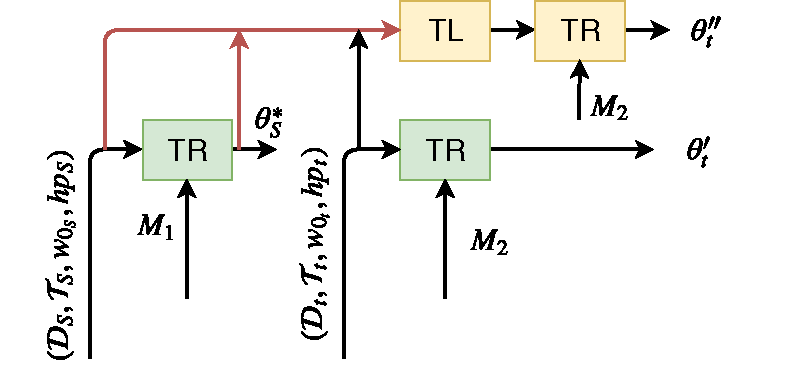
\includegraphics[width = 0.8\textwidth]{figures/transferLearning/TL.pdf}
    \caption[Η διαδικασία μετάδοσης γνώσης]{Η διαδικασία μετάδοσης γνώσης (TL) σε σχέση με την απλή εκπαίδευση (TR) και η σύγκριση της πορείας πληροφορίας. Η μεταβλητή $\theta^*_S$ είναι οι παράμετροι που επιστρέφει η εκπαίδευση στο αρχικό πεδίο ορισμού. Η μεταβλητή $\theta'_t$ είναι οι παράμετροι που επιστρέφει η εκπαίδευση στο τελικό πεδίο ορισμού χωρίς μετάδοση γνώσης. Η μεταβλητή $\theta''_t$ είναι οι παράμετροι που επιστρέφει η εκπαίδευση στο τελικό πεδίο ορισμού με χρήση μετάδοσης γνώσης.}
    \label{fig:TL}
\end{figure}
    


% η συνάρτηση πρόβλεψης έχει πιθανοτικά προσεγγιστεί ως $\hat{f}_s$, $\hat{f}_s(x) = M\left(x; W\right)$.
% Δηλαδή $ \mathtt{Prf}\left(T, \hat{f}\left(\mathcal{X}_{s_{test}}\right)\right) $.


% Δηλαδή $Pr\left(\abs{\hat{f}_s - f_s} >\delta\right) < \epsilon$ για κάποιο $\epsilon$ ικανά μικρό και $\epsilon(\delta) \downarrow$.
% Επίσης έστω ένα πεδίο ορισμού στόχου $\mathcal{D}_t$ και ένα έργο στόχος $ Τ_t $. Αν η συνάρτηση $f_t$ έχει πιθανοτικά προσεγγιστεί ως $\hat{f}_t$ λαμβάνοντας
% υπόψιν μόνο το πεδίο ορισμού στόχο και το έργο στόχο.
% Η μετάδοση γνώσης(Transfer Learning) είναι ένας αλγόριθμος ο οποίος έχει εν γένει είσοδο $(\mathcal{D}_s, T_s, \hat{f}_s, \mathcal{D}_t, T_t)$ και έξοδο μία


Στην παρούσα εργασία $ M_s = M_t = M$, δηλαδή χρησιμοποιείται το ίδιο μοντέλο στην αρχική και στην τελική εκπαίδευση, απλά οι παράμετροί τους δεν είναι ίδιες.

% transfer learning and multi-task learning
\section{Σχέση μετάδοσης γνώσης και μάθησης πολλαπλών έργων}
Η έννοια της μετάδοσης γνώσης είναι πολύ κοντινή με τη μάθηση πολλαπλών έργων (MTL) ταυτοχρόνως. Η MTL χρησιμοποιεί παραλληλισμό των έργων στο ίδιο πεδίο ορισμού. Με αυτό τον τρόπο μοιράζονται χαρακτηριστικά που εξάγονται στο ένα έργο και απαιτούνται στα υπόλοιπα. Στο τέλος αυτής της εκπαίδευσης μπορεί το μοντέλο να έχει καλύτερη επίδοση ακόμα και μόνο σε ένα έργο από ότι αν γινόταν εκπαίδευση μόνο σε αυτό ξεχωριστά. Οι λόγοι για τους οποίους συμβαίνει αυτό δε θα αναλυθούν, ωστόσο για παραπάνω διερεύνηση ο αναγνώστης παραπέμπεται στο \cite{43}. 

Η διαφορά με τη μετάδοση γνώσης είναι ότι η μετάδοση γνώσης λύνει το πρόβλημα σειριακά, μαθαίνοντας πρώτα τα χαρακτηριστικά τα οποία επιλύουν το πρώτο έργο και μετά μεταβαίνει στο επόμενο. Αν όλα τα έργα αφορούν το ίδιο πεδίο ορισμού, τότε η MTL είναι η προτεινόμενη λύση. Ωστόσο, δεν μπορεί να εφαρμοστεί όταν τα έργα αφορούν και διαφορετικά πεδία ορισμού. Αντίθετα, η μετάδοση γνώσης μπορεί να χρησιμοποιήσει χαρακτηριστικά από ένα έργο σε ένα πεδίο ορισμού και έργο $ \mathcal{D}_s, \mathcal{T}_s $ αντίστοιχα, προκειμένου να έχει καλύτερη επίδοση σε ένα πεδίο ορισμού και έργο $ \mathcal{D}_t, \mathcal{T}_t $.

% Present various scenarios
\section{Διάφορα σενάρια μετάδοσης γνώσης }
Παρακάτω δίνεται μία περίληψη των διαφόρων σεναρίων μετάδοσης γνώσης όπως αναφέρονται στα \cite{38} \cite{40}, αλλά με πιο σύγχρονα παραδείγματα.

\subsection{Επαγωγική μετάδοση γνώσης}
% \vspace{1ex}\\
{ \rule{1ex}{1ex} }%
\textit{Δοθέντος ενός αρχικού πεδίου ορισμού $\mathcal{D}_S$ με ένα αρχικό έργο $\mathcal{T}_S$ και ένα τελικό πεδίο ορισμού $\mathcal{D}_t$ με ένα τελικό έργο $\mathcal{T}_t$, η επαγωγική μετάδοση γνώσης αποσκοπεί στη βελτίωση της μάθησης της τελικής συνάρτησης ετικετοποίησης $f_t$ στο τελικό πεδίο ορισμού $\mathcal{D}_t$ χρησιμοποιώντας γνώση από τα $\mathcal{D}_S, \mathcal{T}_S$, όπου $\mathcal{T}_S \neq \mathcal{T}_t$.}

Στον παραπάνω ορισμό τα $\mathcal{D}_S$ και $\mathcal{D}_t$ μπορούν να είναι σχετικά. Βασιζόμενοι στο παραπάνω ορισμό, απαιτούνται μόνο λίγα ετικετοποιημένα δεδομένα για την πρόβλεψη της τελικής συνάρτησης ετικετοποίησης. Γενικά, πρόκειται για πληροφοριοδοτημένη άνευ επίβλεψης μετάδοση γνώσης, όπου εκεί βρίσκεται αρκετό ερευνητικό και πρακτικό ενδιαφέρον. Ωστόσο, υπάρχει και η περίπτωση να είναι Μη-Πληροφοριοδοτημένη άνευ επίβλεψης μετάδοση γνώσης.

% Ένα παράδειγμα της επαγωγικής μετάδοσης γνώσης περιγράφεται στο \cite{46}. Σε αυτό οι συγγραφείς λαμβάνουν ψυχομετρικά δεδομένα από ένα πείραμα εικονικής οδήγησης. Μετά από αυτό το πείραμα δημιουργήθηκε ένα μοντέλο για τη πρόβλεψη του βαθμού διέγερσης του ατόμου. Λαμβάνοντας όλα αυτά, δημιούργησαν ένα καινούριο μοντέλο για την πρόβλεψη της εγκεφαλικής δραστηριότητας και 

\subsubsection{Μεταφορά γνώσης από στιγμιότυπα}
Η μεταφορά στιγμιοτύπων για την επαγωγική μετάδοση γνώσης είναι αρκετά διαισθητική. Αν και η πλειονότητα των δεδομένων του αρχικού πεδίου ορισμού δεν μπορεί να χρησιμοποιηθεί απευθείας, υπάρχουν μέσα σε αυτά μέλη τους τα οποία μπορούν να χρησιμοποιηθούν μαζί με μερικά ετικετοποιημένα δεδομένα του τελικού πεδίου ορισμού.

Για παράδειγμα έχει προταθεί ο αλγόριθμος TrAdaBoost, ο οποίος είναι μία επέκταση του αλγορίθμου AdaBoost, προκειμένου να λύσει τα προβλήματα επαγωγικής μεταφοράς γνώσης. Ο TrAdaBoost υποθέτει ότι το αρχικό και το τελικό πεδίο ορισμού χρησιμοποιούν τις ίδιες ετικέτες και χαρακτηριστικά, αλλά οι κατανομές των δεδομένων στα δύο πεδία ορισμού είναι διαφορετικές. Επιπλέον, ο TrAdaBoost υποθέτει ότι λόγω της διαφοράς των κατανομών, μερικά από τα δεδομένα του αρχικού πεδίου ορισμού μπορεί να βοηθήσουν στην εκπαίδευση στο τελικό πεδίο ορισμού, αλλά μπορεί και να δυσχεραίνουν την εκπαίδευση.

Ο αλγόριθμος προσπαθεί να ζυγιάσει τα δεδομένα προκειμένου να μειώσει τα δεδομένα με αρνητική επίδραση στην εκπαίδευση και να ενισχύσει τα δεδομένα με θετική επίδραση στην εκπαίδευση στο τελικό πεδίο ορισμού. Σε κάθε επανάληψη του, ο TrAdaBoost εκπαιδεύει το βασικό ταξινομητή (συνάρτηση πρόβλεψης - μοντέλο) σε αυτό το ζυγιασμένο σύνολο δεδομένων. Ωστόσο, το σφάλμα υπολογίζεται μόνο στα δεδομένα του τελικού πεδίου ορισμού. Περεταίρω, ο TrAdaBoost ακολουθεί την ίδια στρατηγική με τον AdaBoost για την ανανέωση των λανθασμένα ταξινομημένων δεδομένων στο τελικό πεδίο ορισμού. Ωστόσο, χρησιμοποιείται διαφορετική στρατηγική για την ανανέωση των λανθασμένα ταξινομημένων δεδομένων στο αρχικό πεδίο ορισμού από το αρχικό μοντέλο. Στο \cite{63} δίνεται μία θεωρητική ανάλυση του αλγορίθμου TrAdaBoost.

\subsubsection{Μετάδοση γνώσης της αναπαράστασης χαρακτηριστικών}
Η προσέγγιση με τη μετάδοση της αναπαράστασης χαρακτηριστικών στο πρόβλημα της επαγωγικής μετάδοσης γνώσης σκοπεύει στην εύρεση αναπαραστάσεων χαρακτηριστικών για τη μείωση της απόκλισης των πεδίων ορισμού και του σφάλματος ταξινόμησης ή παλινδρόμησης του μοντέλου. Οι στρατηγικές για την εύρεση τέτοιων αναπαραστάσεων χαρακτηριστικών διαφέρουν μεταξύ τους ανάλογα με το αρχικό πεδίο ορισμού. Αν πολλά ετικετοποιημένα δεδομένα είναι διαθέσιμα στο πεδίο ορισμού, μπορούν να χρησιμοποιηθούν τεχνικές επιβλεπόμενης μάθησης για την εύρεση των χαρακτηριστικών. Αυτό είναι όμοιο με τη συνήθη μάθηση πολλαπλών έργων. Αν δεν υπάρχουν ετικετοποιημένα δεδομένα στο αρχικό πεδίο ορισμού, τότε θα πρέπει να χρησιμοποιηθούν μέθοδοι μη επιβλεπόμενης μάθησης, ώστε να κατασκευασθούν τα χαρακτηριστικά που χρειάζονται για αυτή την προσέγγιση.
\vspace{1em}

\textbf{Παράδειγμα 1ο}\\
Επιβλεπόμενη κατασκευή χαρακτηριστικών:

Όπως επισημάνθηκε παραπάνω οι μέθοδοι επιβλεπόμενης κατασκευής χαρακτηριστικών για την επαγωγική μετάδοση γνώσης είναι όμοιες με αυτές της μάθησης πολλαπλών έργων. Η βασική ιδέα είναι η εκμάθηση μίας χαμηλής διάστασης αναπαράστασης η οποία είναι κοινή μεταξύ σχετικών έργων. Επιπλέον, η καινούρια αυτή αναπαράσταση μπορεί να μειώσει το σφάλμα ταξινόμησης ή παλινδρόμησης του μοντέλου σε κάθε ένα από τα υποψήφια έργα.

Αυτή η προσέγγιση μπορεί να μελετηθεί και ως ένα πρόβλημα βελτιστοποίησης. Σε αυτό τα κοινά χαρακτηριστικά μπορούν να γίνουν γνωστά επιλύοντας το παρακάτω πρόβλημα:
$$
argmin \sum_{t \in \{\mathcal{T}_t, \mathcal{T}_S\} } {\sum_{i=1}^{n_t}} {L\left(y_{t_i}, \langle a_t, U^T x_{t_i} \rangle  \right) + \gamma \|A\|^{2}_{2,1} } 
$$
$$
U \in \mathbf{O}^d
$$
Στην παραπάνω εξίσωση  τα $\mathcal{T}_S$, $\mathcal{T}_t$ δηλώνουν το αρχικό και το τελικό έργο στα αντίστοιχα πεδία ορισμού. Επίσης ο $A = [a_s,a_t] \in R^{d\times2}$ είναι ένας πίνακας των παραμέτρων. Ο $U$ είναι ένας ορθογώνιος πίνακας $d \times d$ που απεικονίζει τα αρχικά δεδομένα υψηλής διάστασης σε αναπαραστάσεις χαμηλής διάστασης. Η νόρμα $(r, p)$ του $A$ ορίζεται ως $ \|A\|_{r,p} = \left( \sum_{i=1}^{d}{\| a^i\|_{p}^{r}} \right)^{\frac{1}{p}}$. Το πρόβλημα αυτό υπολογίζει τις αναπαραστάσεις $U^T X_T$, $U^S X_S$ και τις παραμέτρους, $A$ του μοντέλου ταυτοχρόνως. Το πρόβλημα βελτιστοποίησης μπορεί να μετατραπεί και σε ένα κυρτό πρόβλημα \cite{47}. Η λύση αυτή αναλύεται περισσότερο στο \cite{46}, ωστόσο όπως είναι εύληπτο από τον αναγνώστη θα μπορούσε να χρησιμοποιηθεί και ένα νευρωνικό δίκτυο (όχι απαραίτητα βαθύ) για την επίλυση του προβλήματος.
\vspace{1em}

\textbf{Παράδειγμα 2ο}\\
Άνευ επίβλεψης κατασκευή χαρακτηριστικών:

Ένα πολύ καλό παράδειγμα αυτής της προσέγγιση είναι ο νευρωνικός στατιστικολόγος όπως αναλύεται στο \cite{48}. 
Σύμφωνα με αυτούς, για να μεταφέρει μία μηχανή χαρακτηριστικά από το ένα σύνολο δεδομένων στο άλλο, θα πρέπει να καταλαβαίνει τις ομοιότητες. Για να το πράξει αυτό θα πρέπει να περιγράφει όλο το σύνολο δεδομένων και όχι να περιγράφει τα δεδομένα του απλά ως ανεπεξέργαστα σημεία. Προς αυτό το σκοπό χρησιμοποίησαν και επέκτειναν έναν μεταβλητό αυτόματο κωδικοποιητή \cite{49} για να υπολογίσει στατιστικά ενός συνόλου δεδομένων άνευ επίβλεψης. Οι στατιστικές αυτές μπορούν να χρησιμοποιηθούν για την ομαδοποίηση συνόλων δεδομένων και την ταξινόμηση άγνωστων μέχρι τώρα συνόλων δεδομένων. Ως εκ τούτου και το όνομα του αλγορίθμου, αφού μπορεί να εξάγει στατιστικές των συνόλων δεδομένων άνευ επίβλεψης χρησιμοποιώντας ένα νευρωνικό δίκτυο.

Μία άλλη γνωστή μέθοδος που αναλύει αυτή την περίπτωση είναι η χρήση μάθησης πολλαπλοτήτων.  Σε αυτή την εργασία \cite{50} προτείνεται μία προσέγγιση προκρουστικής ανάλυσης για την διάταξη των πολλαπλοτήτων, η οποία μπορεί να χρησιμοποιηθεί στην μετάδοση γνώσης μεταξύ προβλημάτων.

\subsubsection{Μετάδοση γνώσης των Παραμέτρων}
Οι περισσότερες μέθοδοι μεταφοράς παραμέτρων για την επαγωγική μετάδοση γνώσης υποθέτουν ότι δύο ξεχωριστά ή ίδια μοντέλα για σχετικά έργα θα πρέπει να μοιραστούν κάποιες παραμέτρους ή κατανομές υπερπαραμέτρων. Τα μοντέλα που βρίσκονται υπό αυτή τη μέθοδο συνήθως αφορούν πολλαπλά έργα. Αυτό βέβαια δεν προβάλει κάποιο πρόβλημα, απλά από το να παραλληλισθούν τα δύο πεδία ορισμού, τοποθετώντας ένα μοντέλο, λαμβάνεται το μοντέλο εκπαιδευμένο στο πρώτο πρόβλημα και χρησιμοποιούνται τα δεδομένα εστιάζοντας στην καλύτερη επίδοση του μοντέλου στο δεύτερο (τελικό) πρόβλημα. 

Σε αυτή την κατηγορία υπόκειται και το δίκτυο SqueezeDet. Αρχικά οι ερευνητές που το δημιούργησαν στο πρώτο κομμάτι του που είναι το SqueezeNet έλαβαν όλες τις παραμέτρους από προηγούμενη εκπαίδευση του SqueezeNet στο ImageNet. Αυτή είναι περίπου και η μέθοδος που ακολουθείται στην εργασία. Ωστόσο, αυτή έχει και ερωτήματα όπως: πώς να αποφασίσει κανείς πόσες παραμέτρους να λάβει από μία προηγούμενη εκπαίδευση, ποιες και πόσες παραμέτρους χρειάζεται να επαναεκπαιδεύσει, μήπως υπάρχει κάποια σχέση πως να αλλάξει τις υπερπαραμέτρους με βάσει την απόφαση λήψης των παραμέτρων; Αυτά και άλλα απαντώνται παρακάτω.


\subsection{Μεταγωγική μετάδοση γνώσης}
% \vspace{1ex}\\
{ \rule{1ex}{1ex} }%
\textit{Δοθέντος ενός αρχικού πεδίου ορισμού $\mathcal{D}_S$ με ένα αρχικό έργο $\mathcal{T}_S$ και ένα τελικό πεδίο ορισμού $\mathcal{D}_t$ με ένα τελικό έργο $\mathcal{T}_t$, η μεταγωγική μετάδοση γνώσης αποσκοπεί στη βελτίωση της μάθησης της τελικής συνάρτησης ετικετοποίησης $f_t$ στο τελικό πεδίο ορισμού $\mathcal{D}_t$ χρησιμοποιώντας γνώση από τα $\mathcal{D}_S, \mathcal{T}_S$, όπου $\mathcal{D}_S \neq \mathcal{D}_t$ και $ \mathcal{T}_s = \mathcal{T}_t $. Επιπλέον, θα πρέπει να υφίστανται κάποια μη ετικετοποιημένα δεδομένα στο τελικό πεδίο ορισμού στη διάρκεια της εκπαίδευσης.}

Η έννοια της μεταγωγικής μετάδοσης γνώσης δε θα πρέπει να συγχέεται με την έννοια της μεταγωγικής μάθησης όπου όλα τα δεδομένα ελέγχου πρέπει να είναι γνωστά κατά την εκπαίδευση, η οποία δεν επιτρέπει το μοντέλο να επαναχρησιμοποιηθεί για μελλοντικά δεδομένα. Για να εξάγει αποτελέσματα από τα καινούρια δεδομένα θα πρέπει να τα κατηγοριοποιήσει στις ίδιες κατηγορίες με όλα τα υπάρχοντα. Παρομοίως όμως με τη μεταγωγική μάθηση, στη μεταγωγική μετάδοση γνώσης υποτίθεται ότι υπάρχουν μη ετικετοποιημένα δεδομένα στο τελικό πεδίο ορισμού. 

Στον παραπάνω ορισμό της μεταγωγικής μετάδοσης γνώσης το αρχικό και το τελικό πεδίο ορισμού είναι τα ίδια, το οποίο συνεπάγεται ότι μπορεί η συνάρτηση πρόβλεψης του αρχικού προβλήματος να προσαρμοστεί για το δεύτερο και να χρησιμοποιηθεί για τα μη ετικετοποιημένα δεδομένα στο τελικό πεδίο ορισμού. Η προσαρμογή αυτή υπόκειται σε δύο περιπτώσεις: 1) Οι χώροι των των χαρακτηριστικών των δύο πεδίων ορισμού είναι διαφορετικοί $ \mathcal{X}_S \neq \mathcal{X}_t $ και 2) οι χώροι των χαρακτηριστικών των πεδίων ορισμού είναι ίδιοι, αλλά οι πιθανοτικές κατανομές είναι διαφορετικές: $ P\left(X_S\right) \neq P\left( X_t\right)$.  Αυτό είναι σχεδόν ίδιο με τις απαιτήσεις της προσαρμογής του πεδίου ορισμού και του προβλήματος της πόλωσης των δειγμάτων λόγω δειγματοληψίας.

\subsubsection{Μεταφορά γνώσης από στιγμιότυπα}
Οι προσεγγίσεις αυτού του τύπου βασίζονται κυρίως στη σημασία της δειγματοληψίας. Προκειμένου να δειχθεί η σημασία της επιλογής μεθόδου δειγματοληψίας, παρουσιάζεται το μεγαλύτερο πρόβλημα της μεταφοράς γνώσης από στιγμιότυπα που είναι η ελαχιστοποίηση του εμπειρικού ρίσκου. Γενικότερα, θα ήταν επιθυμητό οι βελτιστοποιημένες παραμέτροι $\theta^*$ του μοντέλου να είναι βελτιστοποιημένες ως προς το αναμενόμενο ρίσκο: 
$$
\theta^* = argmin_{\theta \in \Theta} E_{(x,y) \in P} \left[ l(x, y, \theta)\right]
$$
όπου $l(x, y, \theta)$ είναι η συνάρτηση σφάλματος η οποία εξαρτάται από την παράμετρο $\theta$. Ωστόσο είναι δύσκολο να εκτιμηθεί η κατανομή P. Για αυτό προτιμάται η ελαχιστοποίηση του εμπειρικού ρίσκου:
$$
\theta^* = argmin_{\theta \in \Theta} \frac{1}{n}\sum_{i=1}^{n} \left[ l(x_i, y_i, \theta)\right]
$$
όπου $n$ είναι το μέγεθος των δεδομένων προς εκπαίδευση.

Στη μεταγωγική μετάδοση γνώσης, σκοπός είναι η εύρεση ενός βέλτιστου μοντέλου για το τελικό πεδίο ορισμού δεδομένων ελαχιστοποιώντας το αναμενόμενο ρίσκο:
$$
\theta^* = argmin_{\theta \in \Theta} \sum_{(x,y) \in D_{d_t}} P\left(D_{d_t}\right) l(x, y, \theta)
$$

Αν δεν υπάρχουν ετικετοποιημένα δεδομένα στο τελικό πεδίο ορισμού δεδομένων, τότε θα πρέπει το μοντέλο να εξαχθεί από τα δεδομένα του αρχικού πεδίου ορισμού. Αν $ P(D_{d_S}) = P(D_{d_t}) $, τότε αρκεί να βελτιστοποιηθούν οι παράμετροι του μοντέλου όπως παρακάτω:
$$
\theta* = argmin_{\theta \in \Theta} \sum_{(x,y) \in D_{d_S}} P\left(D_{d_S}\right) l(x, y, \theta).
$$
Διαφορετικά αν $ P(D_{d_S}) \neq P(D_{d_t})$, θα πρέπει να αλλάξει το παραπάνω πρόβλημα βελτιστοποίησης, ώστε το μοντέλο που θα εξαχθεί από την εκπαίδευση να έχει δυνατότητα μεγάλης γενίκευσης στο τελικό πεδίο ορισμού. Η αλλαγή είναι η εξής:
$$
\theta^* = argmin_{\theta \in \Theta} \sum_{(x,y) \in D_{d_S}} \frac{P\left(D_{d_t}\right)}{P\left(D_{d_S}\right)} P\left(D_{d_S}\right) l(x, y, \theta)
$$
$$
	\approx argmin_{\theta \in \Theta} \sum_{i=1}^{n_S} \frac{P_t\left(x_{t_i}, y_{t_i}\right)}{P\left(x_{S_i}, y_{S_i}\right)}  l(x_{S_i}, y_{S_i}, \theta).
$$
Σε αυτή την αλλαγή τοποθετούνται διαφορετικές τιμές ποινής στα στιγμιότυπα $(x_{S_i}, y_{t_i})$ πολλαπλασιάζοντας τα με τα βάρη $\frac{P_t\left(x_{t_i}, y_{t_i}\right)}{P\left(x_{S_i}, y_{S_i}\right)}$. Κατά αυτό τον τρόπο εξάγεται ένα ακριβές μοντέλο για το τελικό πρόβλημα. Επιπρόσθετα, αφού τα έργα είναι κοινά, ισχύει $P\left( Y_t | X_t\right) = P\left(Y_S, X_S\right)$. Επομένως, ο λόγος των κατανομών μπορεί να προσεγγισθεί πιο εύκολα:
$$
 \frac{P\left(x_{t_i}, y_{t_i}\right)}{P\left(x_{S_i}, y_{S_i}\right)} =  \frac{P\left(x_{t_i}\right)}{P\left(x_{S_i}\right)}.
$$
Αν είναι δυνατόν να υπολογιστούν τα $\frac{P_t\left(x_{t_i}\right)}{P\left(x_{S_i}\right)}$ για κάθε στιγμιότυπο, τότε δύναται να επιλυθούν όλα τα προβλήματα που υπόκεινται στην κατηγορία της μεταγωγικής μετάδοσης γνώσης. Στη βιβλιογραφία υπάρχουν διάφοροι τρόποι για τον υπολογισμό του παραπάνω λόγου, ωστόσο ξεφεύγουν από το αντικείμενο αυτής της διπλωματικής.

Ένα άμεσα σχετιζόμενο παράδειγμα είναι η εργασία της \textit{brighter.ai} \cite{54} για τον εντοπισμό αντικειμένων σε εικόνες υπό διαφορετικές συνθήκες. Δηλαδή στα περισσότερα σύνολα δεδομένων για αλγορίθμους εντοπισμού, όπως και στις περισσότερες εκπαιδεύσεις δε λαμβάνονται υπόψη περιπτώσεις που οι καιρικές συνθήκες ή η ώρα της ημέρας δυσχεραίνουν την όραση. Έτσι οι περισσότεροι αλγόριθμοι δεν μπορούν να χρησιμοποιηθούν σε αυτές τις περιπτώσεις.

Για την αντιμετώπιση αυτού του του προβλήματος οι ερευνητές της \textit{brighter.ai} χρησιμοποίησαν 2 νευρωνικά δίκτυα τύπου GAN συνδεδεμένα σειριακά, ώστε να απεικονίσουν τα δεδομένα της μίας συνθήκης στην άλλη κρατώντας τη μορφή των αντικειμένων ώστε να μπορούν να εντοπιστούν. Αν η κατάσταση στην οποία ο αλγόριθμος είναι θεμιτό να λειτουργήσει είναι η νύκτα, τότε: Το πρώτο δίκτυο GAN μετατρέπει την εικόνα από νύκτα σε μέρα και το δεύτερο GAN από μέρα σε νύκτα. Οι ερευνητές τονίζουν τη σημασία του δευτέρου, ώστε να μπορεί να υπάρχει μία ισομορφική απεικόνιση. Επίσης, ως μετρική απόστασης της κατασκευασμένης εικόνας και της πραγματικής από τα δίκτυα GAN χρησιμοποιούν την ευκλείδεια απόσταση μεταξύ των χαρακτηριστικών που εξάγονται κάποιο νευρωνικό δίκτυο κατηγοριοποίησης (πιθανόν εκπαιδευμένο στο αρχικό πεδίο ορισμού) στο αρχικό πεδίο ορισμού και στο τελικό πεδίο ορισμού. Ως σφάλμα προσέγγισης χρησιμοποιούν την απόσταση των εικόνων σε κάθε GAN και ένα άλλο σχεδόν αμετάβλητο χαρακτηριστικό, ανάλογα με τις συνθήκη των εικόνων.Το ίδιο δίκτυο με το οποίο εξήχθησαν τα χαρακτηριστικά, μετά μπορεί να χρησιμοποιηθεί για τον εντοπισμό αντικειμένων.

\subsubsection{Μετάδοση γνώσης της αναπαράστασης χαρακτηριστικών}
Οι περισσότερες μελέτες μεταγωγικής μετάδοσης γνώσης  με τη μεταφορά χαρακτηριστικών, αφορούν αλγορίθμους μηχανικής μάθησης άνευ επίβλεψης. Για την καλύτερη κατανόηση αυτής της μεθόδου παρουσιάζονται δύο αλγόριθμοι.

1ος Αλγόριθμος \cite{52}\\
Νευρωνική μάθηση δομικής αντιστοιχίας:

Σε αυτή την εργασία οι συγγραφείς υιοθέτησαν τη μετάδοση γνώσης με δομική αντιστοιχία \cite{53}, αλλά προτίμησαν την αναζήτηση αυτής να την πραγματοποιήσουν με ένα πιο σύγχρονο τρόπο: τους νευρωνικούς αυτόματους κωδικοποιητές όπως εκθέτουν και οι ίδιοι. Το πρόβλημα βέβαια που επιλύουν αφορά την επεξεργασία της φυσικής γλώσσας (NLP). Αυτό βέβαια, δεν εμποδίζει την περίληψη αυτής της εργασίας στην παρούσα, αφού η αντιστοιχία μοντέλων που επιλύουν προβλήματα αυτού του τομέα με αυτά της τεχνητής όρασης είναι αρκετά συχνή. 

Αρχικά η προσέγγιση αυτή ξεχωρίζει τα χαρακτηριστικά σε αξονικά χαρακτηριστικά (ή χαρακτηριστικά άξονα) και στα υπόλοιπα. Ο διαχωρισμός αυτός γίνεται εκ των προτέρων, δηλαδή πριν την εφαρμογή του αλγορίθμου και αφορά το αρχικό πεδίο ορισμού. Τα αξονικά χαρακτηριστικά δίνονται ως υπέρ-παράμετροι στον αλγόριθμο και έπειτα αυτός αποφασίζει κατά πόσο εφικτή είναι η περιγραφή των υπολοίπων χαρακτηριστικών από αυτά τα αξονικά χαρακτηριστικά. 

Η αρχιτεκτονική της λύσης αναλύεται καλύτερα μέσω του Σχήματος \ref{fig:SCL_autoencoder}. Εκεί διακρίνονται οι διαφορές μεταξύ ενός απλού αποκωδικοποιητή και αυτής της μεθόδου. Όπως παρατηρείται και στην εργασία της νευρωνικής μάθησης δομικής αντιστοιχίας, είναι η πρώτη φορά που χρησιμοποιείται η αρχιτεκτονική του αυτόματου αποκωδικοποιητή για αυτό το σκοπό και για αυτό δεν χρησιμοποιήθηκε και κάποιος βαθύς κωδικοποιητής ή αποκωδικοποιητής.

\begin{figure}[H]
\centering
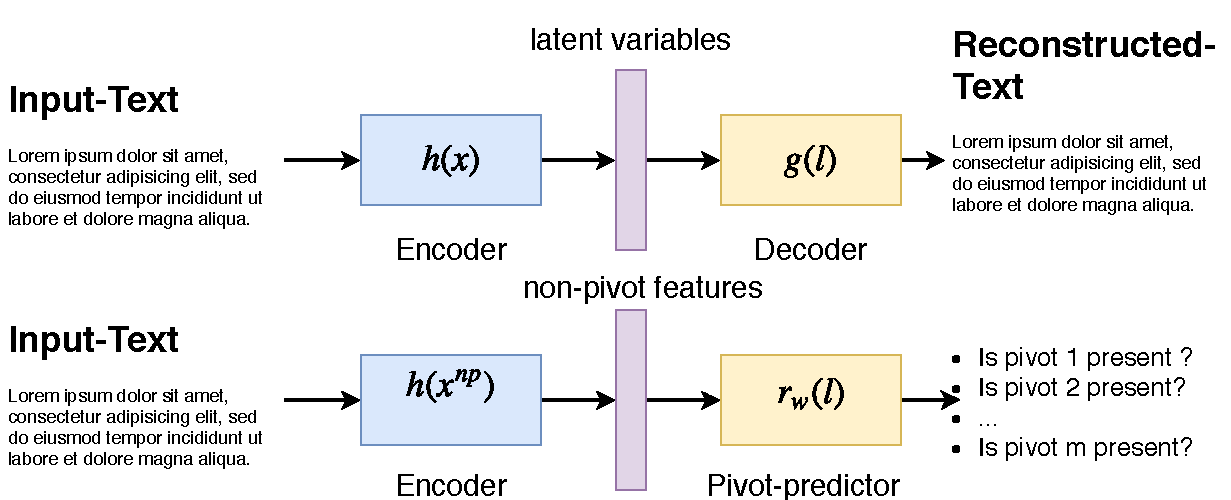
\includegraphics[width = \textwidth]{figures/transferLearning/SCL_autoencoder.pdf}
\caption[Αρχιτεκτονική νευρωνικής μάθησης δομικής αντιστοιχίας]{Στο πάνω μέρος της εικόνας βρίσκεται ένας απλός αυτόματος κωδικοποιητής. Στο κάτω μέρος της εικόνας βρίσκεται ο αυτόματος κωδικοποιητής αλλαγμένος στο κομμάτι του αποκωδικοποιητή όπως προβλέπει ο αλγόριθμος. Στο τέλος δε γίνεται ανακατασκευή της εισόδου, αλλά δίνεται η απάντηση αν κάποιο από τα αξονικά χαρακτηριστικά υπάρχει στην έξοδο του κωδικοποιητή. Το $x$ και το αποτέλεσμα της συνάρτησης $h(x^{np})$ είναι δυαδικά διανύσματα. Η βελτιστοποίηση γίνεται χρησιμοποιώντας τη συνάρτηση απόκλισης \textit{Kullback-Leibler}.}
\label{fig:SCL_autoencoder}
\end{figure}

2ος αλγόριθμος\\
Transfer Component Analysis (TCA):
Ο αλγόριθμος αυτός ουσιαστικά εξάγει χαρακτηριστικά από τα δύο πεδία ορισμού, θεωρώντας ότι όλα τα κοινά χαρακτηριστικά ανήκουν σε έναν αναπαραγόμενο χώρο πυρήνων Hilbert (RKHS). Τα δύο δεδομένα που λαμβάνει υπόψη του ο αλγόριθμος είναι ότι : $ P(X_S) \neq P(X_t)$ και $P(Y_S|X_S) = P(Y_t|X_t)$. Έπειτα θεωρώντας ότι υπάρχει μία λανθάνουσα απεικόνιση $\phi : \mathcal(X)\rightarrow mathcal(H)$ για τα $X_S$, $X_t$ η οποία είναι ισομορφισμός και ουσιαστικά δημιουργεί τα χαρακτηριστικά των δύο πεδίων ορισμού, ψάχνει αυτήν τη συνάρτηση $\phi$ η οποία ελαχιστοποιεί τη μετρική μέγιστης μέσης ασυμφωνίας(MMD):
$$
Dist(X_S’,X_t’) = \| \frac{1}{n_1} \sum_{i=1}^{n_1}\phi(x_{S_i}) -  \frac{1}{n_2} \sum_{i=1}^{n_2}\phi(x_{t_i}) \|_{\mathcal{H}}
$$
$$
\phi^* = argmin_{\phi} Dist(X_S’,X_t’)
$$
Σε αυτό το σημείο κάνει τη θεώρηση κλειδί αυτής της εργασίας, ότι $ P(Y_S|\phi(X_S)) = P(Y_t|\phi(X_t))$. Με αυτό και χρησιμοποιώντας το “κόλπο πυρήνα” $k(x_i,x_j) = \phi(x_i)^{T}\phi(x_j)$ οδηγείται στον υπολογισμό της μετρικής μέσω του πίνακα $K$:
$$
Dist(X_S’,X_t’) = tr(KL), \, K =\left[ \begin{matrix} K_{S,S} & K_{S,t}\\ K{t,S} & K_{t,t}\end{matrix}\right] , \, L_{ij} = \frac{1}{n_i n_j}, \, n_i = \left\{ \begin{matrix} n_1 \;\text{if}\. x_i \in X_S\\ n_2 \;\text{if}\; x_i \in X_t \end{matrix} \right.
$$

Βέβαια για τον υπολογισμό του K απαιτείται η λύση μέσω αλγορίθμων SDP και η μετέπειτα επεξεργασία της λύσης μέσω PCA για τη μείωση της διάστασης των χαρακτηριστικών. Αυτό οδηγεί σε μεγάλη πολυπλοκότητα και απώλεια πληροφορίας. Οπότε προτείνεται ο ορισμός ενός δευτέρου πίνακα μέσω της εξίσωσης $ K = \left(K K^{-1/2}\right) \left(K^{-1/2} K\right) $:
$$
\tilde{K} = \left(K K^{-1/2} \tilde{W}\right) \left(\tilde{W}^{T} K^{-1/2} K\right) = KWW^{T}K,\, W = K^{-1/2}\tilde{W} 
$$
οδηγώντας στη μετρική:
$$
Dist(X_S’, X_T’) = tr\left( (KWW^{T}K)L \right) = tr\left( W^{T}KLKW\right)
$$
Η οποία επιλύεται καλύτερα μέσω της αναζήτησης:
$$
W* = argmin_{W} \left[ tr(W^{T}W) + \mu tr\left( W^{T}KLKW\right) \right], \, W^{T}KLKW = I
$$
$$
H = I_{n_1+n_2} - \frac{1}{n_1+n_2} \mathbf{1}_{n_1+n_2,n_1+n_2}
$$
με $\mu$ ορισμένη ως παράμετρος συμβιβασμού. Το σύμβολο $\mathbf{1}_{n,m}$ είναι ένας πίνακας $n\times m$ με όλα τα στοιχεία του ίσα με 1. Η λύση αυτή δίνει πολυπλοκότητα $\mathrm{O}\left(m(n_1+n_2)^{2}\right)$.


\subsubsection{Μετάδοση γνώσης των Παραμέτρων}
Προφανώς στην μεταγωγική μετάδοση γνώσης δεν μπορεί να υπάρξει μετάδοση της γνώσης των παραμέτρων, διότι τα πεδία ορισμού είναι διαφορετικά. Για καλύτερη κατανόηση παρουσιάζεται ένα παράδειγμα: Αν ένα μοντέλο είναι εκπαιδευμένο σε δεδομένα εικόνων σε πολικές συντεταγμένες, τότε δεν μπορούν να χρησιμοποιηθούν οι παράμετροι του για την επίλυση του ίδιου προβλήματος σε καρτεσιανές, απλά μεταφέροντας κάποιες παραμέτρους. Ούτε βέβαια, μπορεί να βοηθηθεί γιατί τα μετέπειτα επίπεδα του μοντέλου με πιο υψηλής διάστασης χαρακτηριστικά βασίζονται στα προγενέστερα επίπεδα με χαμηλότερης διάστασης χαρακτηριστικά τα οποία είναι βασισμένα σε πολικές συντεταγμένες.

\subsection{Άνευ επίβλεψης μετάδοση γνώσης}
% \vspace{1ex}\\
{ \rule{1ex}{1ex} }%
\textit{Δοθέντος ενός αρχικού πεδίου ορισμού $\mathcal{D}_S$ με ένα αρχικό έργο $\mathcal{T}_S$ και ένα τελικό πεδίο ορισμού $\mathcal{D}_t$ με ένα τελικό έργο $\mathcal{T}_t$, η άνευ επίβλεψης μετάδοση γνώσης αποσκοπεί στη βελτίωση της μάθησης της τελικής συνάρτησης ομαδοποίησης ή περιγραφής των δεδομένων $f_t$ στο τελικό πεδίο ορισμού $\mathcal{D}_t$ χρησιμοποιώντας γνώση από τα $\mathcal{D}_S, \mathcal{T}_S$, όπου $\mathcal{T}_S \neq \mathcal{T}_t$ και τα $Y_S, Y_t$ είναι μη παρατηρήσιμα.}

Παρομοίως με τους ορισμούς που έχουν δοθεί στην απλή εκπαίδευση, η άνευ επίβλεψης μετάδοση γνώσης αφορά αρχικό και τελικό έργο χωρίς ορισμένες τις ετικέτες, δηλαδή χωρίς αυστηρά ορισμένη (ή είναι άγνωστη) συνάρτηση ετικετοποίησης. Ωστόσο υπάρχουν και άλλοι ορισμοί οι οποίοι πλαισιώνουν καλύτερα αυτό τον ορισμό υποκατηγοριοποιώντας τον σε συγκεκριμένα σενάρια. Σύμφωνα με τον Cook \cite{44} υπάρχουν τέσσερις κατηγορίες 
\begin{itemize}
    % \item IS: Πληροφοριοδοτημένη υπό επίβλεψη μετάδοση γνώσης, όπου η συνάρτηση ετικετοποίησης είναι γνωστή τόσο στο αρχικό έργο, όσο και στο τελικό.
    \item IU: Πληροφοριοδοτημένη άνευ επίβλεψη μετάδοση γνώσης, όπου η συνάρτηση ετικετοποίησης είναι γνωστή μόνο στο αρχικό έργο.
    \item US: Μη-πληροφοριοδοτημένη υπό επίβλεψη μετάδοση γνώσης, όπου η συνάρτηση ετικετοποίησης είναι γνωστή μόνο στο τελικό έργο.
    \item UU: Μη-Πληροφοριοδοτημένη άνευ επίβλεψη μετάδοση γνώσης, όπου η συνάρτηση ετικετοποίησης είναι άγνωστη τόσο στο αρχικό έργο, όσο και στο τελικό.
\end{itemize}

Διάφορες μέθοδοι έχουν αναπτυχθεί για την επίτευξη αποτελεσμάτων σε αυτές τις τέσσερις κατηγορίες. Η άνευ επίβλεψης μετάδοση γνώσης ονομάζεται και μάθηση μηδενικής λήψης (zero-shot learning). Οι εργασίες που αφορούν τη μάθηση μηδενικής λήψης προσπαθούν να απεικονίσουν το αρχικό πεδίο ορισμού στο τελικό και χρησιμοποιώντας αυτή την απεικόνιση να εκπαιδεύσουν ευκολότερα το μοντέλο στο τελικό πεδίο ορισμού. Για παράδειγμα αυτό θα μπορούσε να γίνει ακόμα και για ένα SVM \cite{45}. Παρόλα αυτά, σε όλες τις προσεγγίσεις συνεχίζουν να ισχύουν οι περιορισμοί των μεθόδων μάθησης άνευ επίβλεψης.

Αυτή η περίπτωση κυρίως περιλαμβάνει τη μεταφορά ομαδοποίησης από το αρχικό πεδίο ορισμού στο τελικό, ή την κατασκευή της τελικής ομαδοποίησης μέσω της τελικής. Η περίπτωση αναφέρεται απλά για πληρότητα. Για ένα παράδειγμα αυτής της μεθόδου ο αναγνώστης παραπέμπεται στον αλγόριθμο STC(αυτοδίδακτη ομαδοποίηση) \cite{53}.

\section{Μεταφερσιμότητα παραμέτρων νευρωνικών δικτύων επεξεργασίας εικόνας \cite{55}}
\label{section:transferability}
Όπως έχει παρουσιαστεί στην εργασία των ερευνητών του KTH \cite{56}, τα χαρακτηριστικά των εικόνων είναι αρκετά κοινά· επομένων μπορούν οι ίδιοι οι παράμετροι να μεταφερθούν από τον έναν αλγόριθμο στον άλλο με αρκετά καλό αποτέλεσμα και υποδιαιρώντας αρκετά τον χρόνο εκπαίδευσης. Επίσης, οι ίδιοι ερευνητές έδειξαν πως απλά προσθέτοντας ένα \textit{svm} στην κορυφή του δικτύου κρατώντας όλο το υπόλοιπο ίδιο και ανεκπαίδευτο στο τελικό πεδίο ορισμού, ήταν εφικτό τα ξεπεράσουν σχεδόν όλα τα αποτελέσματα των αλγορίθμων εκείνης της χρονικής περιόδου.

Όποτε γεννήθηκε ένα καινούριο ερώτημα στους ερευνητές, κατά πόσο αυτή η τεχνική είναι εφικτή, δηλαδή κατά πόσο είναι μεταφέρσιμοι οι παράμετροι των νευρωνικών δικτύων που επεξεργάζονται εικόνες \cite{55}. Όπως αναφέρουν ότι έχουν παρατηρήσει: τα πρώτα επίπεδα κάθε νευρωνικού δικτύου είναι ίδια, αφού πρόκειται για φίλτρα \textit{Gabor}· αυτό μάλιστα είναι συμβατό με την περίπτωσή μας διότι στις μετεκπαιδεύσεις του \textit{SqueezeDet} σε καινούρια σύνολα δεδομένων, τα αρχικά επίπεδα είχαν παραγώγους σφάλματος όπως φαίνεται στο Σχήμα \ref{fig:conv1_vs_conv12_biases_gradients}.

Προκειμένου να απαντήσουν οι ερευνητές στο ερώτημα, πραγματοποίησαν το εξής πείραμα: Λαμβάνοντας ως δίκτυο το AlexNet, πρώτα χώρισαν το ImageNet \cite{56}, με βάση τις κλάσεις του, σε δύο ξεχωριστά σύνολα δεδομένων(πεδία ορισμού) A, B και σε αυτά εκπαίδευσαν ξεχωριστά το δίκτυο, με αποτέλεσμα το δίκτυα Anet, Bnet αντίστοιχα. Ο χωρισμός έγινε με τέσσερις διαφορετικούς τυχαίους τρόπους. Έτσι δοκίμασαν την εκπαίδευση του AlexNet στο σύνολο δεδομένων B με τέσσερις διαφορετικούς τρόπους:

\begin{enumerate}

\item Στα $n$ πρώτα επίπεδα μεταφέρθηκαν παράμετροι από το Anet και αυτά έμειναν μη-εκπαιδεύσιμα, ενώ τα υπόλοιπα εκπαιδεύσιμα.

\item Στα $n$ πρώτα επίπεδα μεταφέρθηκαν παράμετροι από το Anet και όλα τα επίπεδα ήταν εκπαιδεύσιμα. Αυτό καλείται στην εργασία αυτή τελειοποίηση(\textit{fine-tuning}) των μεταφερόμενων παραμέτρων.

\item Στα $n$ πρώτα επίπεδα μεταφέρθηκαν παράμετροι από το Βnet και αυτά έμειναν μη-εκπαιδεύσιμα, ενώ τα υπόλοιπα εκπαιδεύσιμα.

\item Στα $n$ πρώτα επίπεδα μεταφέρθηκαν παράμετροι από το Βnet και όλα τα επίπεδα ήταν εκπαιδεύσιμα. Αυτό καλείται στην εργασία αυτή ως τελειοποίηση των μεταφερόμενων παραμέτρων.

\end{enumerate}

Οι δύο τελευταίες περιπτώσεις, έγιναν για να δείξουν ότι τα επίπεδα εξαρτώνται μεταξύ τους και κατά την εκπαίδευση έχουν εύθραυστη συν-προσαρμογή στα χαρακτηριστικά. Αυτό σημαίνει ότι για να γίνει σωστά η μετάδοση γνώσης δεν μπορεί να επιλεχθεί ο παραπάνω αριθμός $n$ χωρίς πρότερα να εξετασθούν οι αριθμοί $n-1$, $n+1$. Αυτό εξηγεί και την πτώση της έντονα κόκκινης γραμμής στο Σχήμα \ref{fig:net_transferability_results}. Τα αποτελέσματα που εξήγαγαν σε αυτό το Σχήμα φαίνεται να είναι θετικά για την περίπτωση της μεταφοράς με τελειοποίηση των παραμέτρων βελτιώνοντας την γενικότητα των χαρακτηριστικών. Επίσης, φαίνεται ότι τα τελευταία επίπεδα έχουν πιο ειδικά χαρακτηριστικά, ενώ τα πρώτα γενικότερα με αποτέλεσμα όταν το $n$ πλησιάζει μεγάλες τιμές η ακρίβεια του δικτύου στο σύνολο B να γίνεται αρκετά μικρότερη.

Σε επόμενο πείραμα οι ερευνητές προχώρησαν και χώρισαν το ImageNet πάλι σε δύο ξεχωριστά σύνολα A, B όπως πριν, αλλά με τη διαφορά ότι οι κλάσεις θα ήταν αρκετά διαφορετικές μεταξύ τους και όχι τυχαίες (για A είχαν το σύνολο των αντικειμένων κατασκευασμένων από τον άνθρωπο και για Β είχαν το σύνολο πραγμάτων που βρίσκονται στη φύση). Και από αυτό το πείραμα κατέληξαν ότι τα χαρακτηριστικά συνεχίζουν να είναι γενικά και ότι είναι προτιμότερο να χρησιμοποιήσει κανείς αυτά τουλάχιστον στα πρώτα επίπεδα από ότι να κάνει εξολοκλήρου την εκπαίδευση στο σύνολο B.


\begin{figure}
\centering
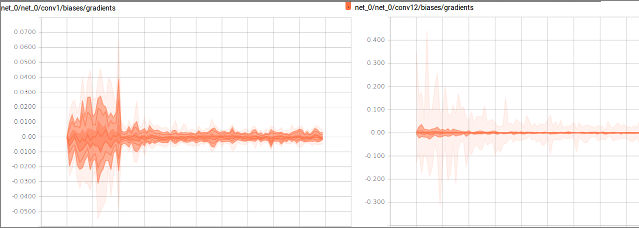
\includegraphics[width = \textwidth]{figures/transferLearning/conv1_vs_conv12_biases_gradients.png}
\caption[Οι κατανομές των παραμέτρων του πρώτου και του τελευταίου επιπέδου]{Η κατανομή της παραγώγου σφάλματος των παραμέτρων πόλωσης του πρώτου επιπέδου φαίνεται να έχει χαμηλότερα μέγιστα από ότι αυτές του τελευταίου επιπέδου κατά τάξη μεγέθους, δείχνοντας ότι το πρώτο επίπεδο του \textit{SqueezeNet}/\textit{SqueezeDet} είναι σχεδόν το ίδιο για τη μετεκπαίδευση στο τελικό πεδίο ορισμού PASCAL VOC2012 \cite{57} και στο αρχικό πεδίο ορισμού ImageNet.}
\label{fig:conv1_vs_conv12_biases_gradients}
\end{figure}

\begin{figure}
\centering
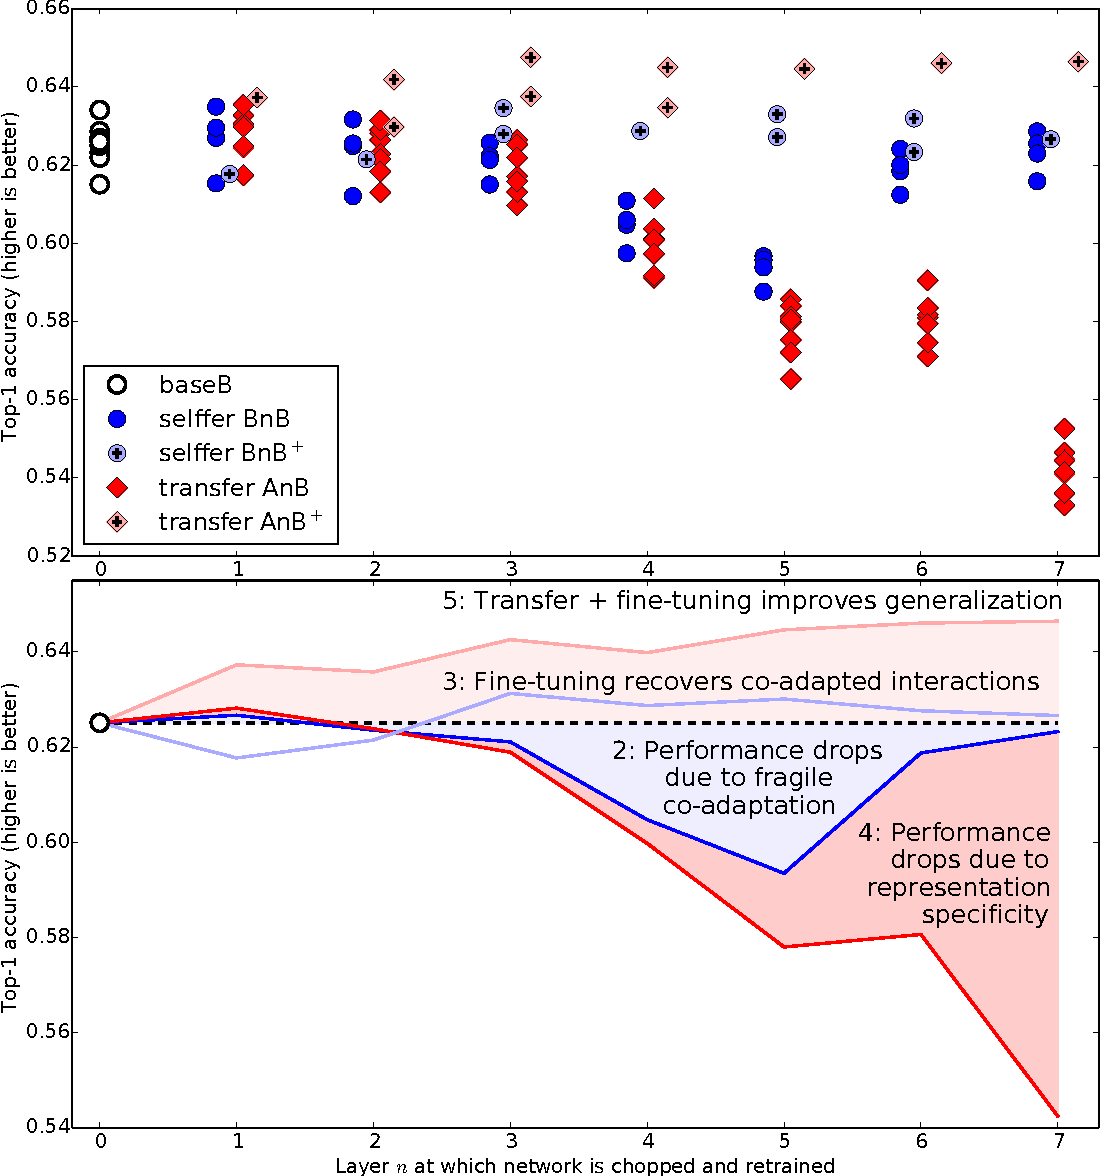
\includegraphics[width = \textwidth]{figures/transferLearning/net_transferability_results.png}
\caption[Τα αποτελέσματα της μετάδοσης γνώσης από το πείραμα μεταφερσιμότητα παραμέτρων]{Πάνω: Κάθε σήμανση στο σχήμα δείχνει τη μέση ακρίβεια στο σύνολο ελέγχου για το εκπαιδευμένο δίκτυο. Οι άσπροι κύκλοι στο $n=0$ δείχνουν την ακρίβεια του Bnet. Υπάρχουν οχτώ σημεία κάθε σήμανσης για κάθε $n$, διότι ελέγχθηκαν 4 διαφορετικοί τυχαίοι διαχωρισμοί του ImageNet. Κάθε κλειστός μπλε κύκλος παρουσιάζει την περίπτωση 3, ενώ κάθε μπλε κύκλος με σταυρό παρουσιάζει το 4. Κάθε κόκκινος ρόμβος παρουσιάζει την περίπτωση 1, ενώ κάθε κόκκινος ρόμβος με σταυρό παρουσιάζει την περίπτωση 2.  Κάτω: Οι γραμμές που συνδέουν τα μέσα του πάνω διαγράμματος για κάθε μία από τις 4 περιπτώσεις. Οι αριθμοί και τα κείμενα στην εικόνα επισημαίνουν το λόγο αυτής της συμπεριφοράς.}
\label{fig:net_transferability_results}
\end{figure}


\section{Αρνητική μετάδοση Γνώσης}
Ήδη από το πείραμα της προηγούμενης παραγράφου είναι κατανοητό ότι υπάρχουν όρια στη μεταφερσιμότητα των παραμέτρων. Όσο πιο διαφορετικά είναι το αρχικό με το τελικό πεδίο ορισμού, τόσο πιο δύσκολο είναι για το νευρωνικό να προσαρμοστεί. Μάλιστα, το πόσο μπορεί να προσαρμοστεί ένας αλγόριθμος έχει και θεωρητικό όριο στην περίπτωση που είναι μορφής Bayes με βάση την πολυπλοκότητα Kolmogorov \cite{61}. 

Αυτά όλα, είναι αρκετά για να φανταστεί κανείς την περίπτωση της αρνητικής μετάδοσης γνώσης, η οποία συμβαίνει “όταν η μεταφορά γνώσης από το αρχικό στο τελικό πρόβλημα προκαλεί μείωση της επίδοσης του αλγορίθμου” \cite{58}. Αυτό μπορεί να συμβαίνει για τρεις λόγους:
\begin{itemize}
\item Λάθος πληροφορία: Αν ο αλγόριθμος μετάδοσης γνώσης, αφαιρεί πληροφορία από το πρώτο πρόβλημα, την οποία θεωρεί ως επιβλαβούσα για την τελική εκπαίδευση, τότε η εκπαίδευση δεν είναι καλύτερη από την περίπτωση που ο αλγόριθμος εκπαιδευόταν μόνο στο τελικό πρόβλημα.
\item Επιλογή αρχικού έργου: Αν υπάρχει παραπάνω από μία επιλογή για το αρχικό σύνολο, ο αλγόριθμος μετάδοσης γνώσης υπάρχει περίπτωση να μην επιλέξει το βέλτιστο ή να διαλέξει να μην επιλέξει κανένα. Για την καλύτερη εικόνα επιλογής αρχικού προβλήματος, ο Eaton \cite{59} πρότεινε τη δημιουργία ενός γράφου όπου η απόσταση κάθε κόμβου από τους υπόλοιπους είναι ίση με μία μετρική μεταφερσιμότητα, όπως φαίνεται στο Σχήμα \ref{fig:transferability_graph}.
\item Ανομοιότητα στο αρχικό και το τελικό έργο: Αν αυτά τα δύο έργα είναι πολύ διαφορετικά, τότε υπάρχει μεγαλύτερο ρίσκο στην μεταγωγική μετάδοση γνώσης να προκληθεί μεγαλύτερο σφάλμα λόγω χρήσης της γνώσης του αρχικού προβλήματος. Αυτό συμβαίνει γιατί όσο πιο όμοια είναι δύο έργα, τόσο πιο κοινά είναι τα χαμηλών διαστάσεων χαρακτηριστικά τους \cite{60}.
\end{itemize}

\begin{figure}[H]
\centering
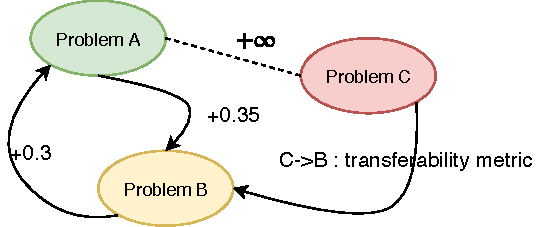
\includegraphics[width = \textwidth]{figures/transferLearning/transferability_graph.pdf}
\caption[Γράφος μεταφερσιμότητας]{Κατευθυνόμενος γράφος όπου κάθε κόμβος είναι ένα πρόβλημα με το δικό του έργο και το δικό του πεδίο ορισμού και κάθε ακμή έχει βάρος τη μετρική μεταφερσιμότητας από το αρχικό πρόβλημα προς το τελικό. Αυτός ο γράφος δεν παρουσιάζεται με αυτό το σχήμα στην εργασία \cite{59}, ωστόσο αυτό εννοείται. Επίσης επιβάλλεται να είναι κατευθυνόμενος λόγω της καταστροφικής \textit{λήθης}.}
\label{fig:transferability_graph}
\end{figure}

\section{Καταστροφική λήθη \cite{62}}
\label{section:catastrophicForgetting}
Τα νευρωνικά δίκτυα είναι κυρίως εμπνευσμένα από τη βιολογία του εγκεφάλου των θηλαστικών, ο οποίος εμπεριέχει νευρώνες οι οποίοι μαθαίνουν και εκπαιδεύονται σε καινούρια προβλήματα καθ’ όλη τη διάρκεια της ζωής του ατόμου. Αυτό σημαίνει ότι αν κάποιο άτομο μάθει να επιλύει ένα πρόβλημα δεν αποκλείει να μάθει την επίλυση ενός άλλου τουλάχιστον σε σύντομο χρονικό διάστημα. Δηλαδή, οι νευρώνες έχουν ελαστικότητα ως προς τη μάθηση.

Η παρατήρηση που έκαναν οι ερευνητές στο \cite{62} είναι ότι αυτό δε συμβαίνει μέχρι τώρα στις εκπαιδεύσεις των νευρωνικών δικτύων. Αυτό που συμβαίνει στην εφαρμογή της μετάδοσης γνώσης ή και στην απλή εκπαίδευση είναι ότι η βελτίωση της επίδοσης γίνεται μόνο για το αρχικό ή το τελικό πρόβλημα και αν έστω μία σειρά προβλημάτων όπως στο Σχήμα \ref{fig:transferability_graph} η διαδρομή $C\rightarrow B\rightarrow A$ δεν είναι εφικτή, διότι η μετάδοση γνώσης από το C στο B και η εκπαίδευση στο πρόβλημα B δεν επιτρέπουν το δίκτυο να ξανά-προσαρμοστεί στο A. Ωστόσο αν υπάρχουν δύο τέλειες λύσεις για τα προβλήματα A, B, τότε αυτές είναι κοντά όπως φαίνεται στο Σχήμα \ref{fig:elasticity_problem}, αλλά ο χώρος στον οποίο η μία λύση πρέπει να ανήκει για να είναι προσβάσιμη από την άλλη διαμέσου του μοντέλου είναι σε μία περιοχή γύρω από τη τέλεια λύση και όχι πάνω σε αυτή. 

Οπότε, είναι θεμιτό να υπολογιστεί αυτή η περιοχή. Ο υπολογισμός αυτής εξαρτάται από τα δεδομένα από ένα υποσύνολο  $\mathcal{D}$ του πεδίου ορισμού. Αν δηλαδή $\theta$ είναι οι παράμετροι του μοντέλου, τότε η πιθανότητα αυτή να είναι η τέλεια λύση για το πεδίο ορισμού $D$ είναι με βάση τον κανόνα Bayes:
$$
\\log p\left(\theta | \mathcal{D} \right) =  \log p\left( \mathcal{D}| \theta \right) + \log p\left(\theta \right) - \log p\left(\mathcal{D} \right)
$$
Οπότε αν συμβαίνει μεταφορά δεδομένων από το πρόβλημα A στο B, η πιθανότητα η $\theta$ να είναι η τέλεια λύση για κάποιο υποσύνολο δεδομένων $\mathcal{D}$:
$$
\log p\left(\theta | \mathcal{D} \right) =  \log p\left( \mathcal{D}_B| \theta \right) + \log p\left(\theta | \mathcal{D}_A\right) - \log p\left(\mathcal{D}_B \right)
$$
Η πραγματική πιθανότητα $ \log p\left(\theta | \mathcal{D}_A\right)$ είναι μη παρατηρήσιμη, οπότε αυτή προσεγγίζεται με μία κατανομή Gauss με μέση τιμή τις βέλτιστες παραμέτρους για το πρόβλημα A: $\theta^*_A$ και με τη διαγώνιο του πίνακα ακρίβειας ίση με τη διαγώνιο του πίνακα πληροφορίας Fisher. Το αποτέλεσμα είναι ότι προκειμένου να γίνουν οι νευρώνες πιο ελαστικοί κατά την εκπαίδευση στο πρόβλημα B μπορεί να χρησιμοποιηθεί η μετρική:
$$
\mathcal{L\left(\theta \right)} = \mathcal{L}_{B}\left(\theta \right) + \sum_{i} \frac{\lambda}{2} F_i\left( \theta_i - \theta^*_{A,i}\right)^2
$$
όπου $\mathcal{L}_{B}\left(\theta \right)$ είναι το σφάλμα κατά την εκπαίδευση στο πρόβλημα B, λαμβάνοντας μόνο υπόψη το πεδίο ορισμού και το έργο του B.


\begin{figure}[H]
\centering
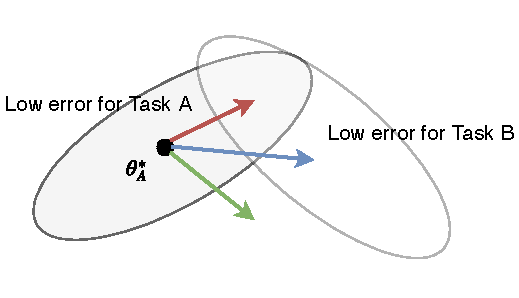
\includegraphics[width = \textwidth]{figures/transferLearning/elasticity_problem.pdf}
\caption[Αλγόριθμος EWC]{Ο αλγόριθμος EWC όπως προτείνεται στο \cite{62}. Προβάλλονται οι περιοχές στις οποίες η λύση είναι ικανοποιητική για τα δύο προβλήματα A,B. Επίσης, δείχνεται ποια η διαφορά μεταξύ των τριών σφαλμάτων: Με \textcolor{Maroon}{κόκκινο} η προτεινόμενη μετρική οδηγεί σε μία περιοχή των παραμέτρων η οποία έχει κοινά ικανοποιητικό σφάλμα. Με \textcolor{blue}{μπλε} η μετρική που δεν έχει βάρος ως προς το μέτρο των παραμέτρων εξέρχεται από την περιοχή της κοινά ικανοποιητικής λύσης. Με \textcolor{SeaGreen}{πράσινο} αν η μετρική σφάλματος λαμβάνει υπόψη το μέτρο των παραμέτρων χρησιμοποιώντας την ευκλείδεια απόσταση αυτών, μπορεί να οδηγηθεί εντελώς εκτός των δύο περιοχών.}
\label{fig:elasticity_problem}
\end{figure}

\section{Προσβασιμότητα}
 Με βάση τη θεωρία αυτομάτου ελέγχου, το παραπάνω πρόβλημα μπορεί να αντιστοιχηθεί σε πρόβλημα προσβασιμότητας. Η προσέγγιση αυτή γίνεται γιατί πιθανόν αυτή να συνδέει περισσότερο τη θεωρία που διδάσκεται ένας ηλεκτρολόγος μηχανικός με το αντικείμενο της μετάδοσης γνώσης. Οι ορισμοί από τη θεωρία προσβασιμότητας είναι οι εξής:
\vspace{1ex}\\
{ \rule{1ex}{1ex} }%
Δοθέντος ενός συστήματος $S(x,u,t)$ και μίας αρχικής κατάστασης $x_0$, η κατάσταση $x_f$ θεωρείται προσβάσιμη από την $x_0$ με είσοδο $u(t)$ αν το σύστημα εντός πεπερασμένου χρόνου $t_f$ μπορεί να μεταβεί από την κατάσταση $x_0$ στην κατάσταση $x_f$.

Επίσης, υπάρχει και ο χρήσιμος ορισμός του προσβάσιμου συνόλου:
\vspace{1ex}\\
{ \rule{1ex}{1ex} }%
Δοθέντος ενός συστήματος $S(x,u,t)$ και μίας αρχικής κατάστασης $x_0$, όλες οι καταστάσεις $x_j$ οι οποίες είναι προσβάσιμες δημιουργούν το προσβάσιμο σύνολο $R^{S}(x_0) = \{z\in X:x_{0}\rightarrow z \}$.
\vspace{1ex}\\
{ \rule{1ex}{1ex} }%
Αν $\Theta$ είναι η περιοχή με ικανοποιητική επίδοση, το αδιέξοδο σύνολο ορίζεται ως $N(S,\Theta) = \{z \in X: R^S(z)\cap \Theta \}$.

Στον παραπάνω ορισμό το αδιέξοδο σύνολο είναι δηλαδή οι καταστάσεις από τις οποίες δεν είναι εφικτή η μετάβαση στο σύνολο $\Theta$.
Έτσι, μπορεί να θεωρηθεί ότι η μετάδοση γνώσης είναι η χρήση προηγούμενων παραμέτρων ή ο μετασχηματισμός του χώρου εισόδου, ώστε το προσβάσιμο σύνολο να εμπεριέχει την περιοχή με το ικανοποιητικό σφάλμα ή να μετακινηθεί η αρχική θέση $x_0$ με αποτέλεσμα το καινούριο προσβάσιμο σύνολο να εμπεριέχει περιοχή με ικανοποιητικό σφάλμα. 

Στην κλασική μηχανική μάθηση όπου η εκπαίδευση γίνεται από την αρχή στο καινούριο πρόβλημα, δημιουργούνται τα εξής προβλήματα:
\begin{itemize}
    \item Έστω ότι γίνεται τυχαία επιλογή των παραμέτρων του μοντέλου $S$ με βάση κάποια συνάρτηση αθροιστικής κατανομής P. Αν η περιοχή με ικανοποιητική επίδοση είναι η $\Theta$, τότε η αρχική κατάσταση των παραμέτρων μπορεί να βρεθεί στο αδιέξοδο σύνολο $N(S,\theta)$, διότι εν γένει δεν ισχύει $P\left( N(S,\Theta)\right) = 0$. Οπότε, μπορεί να χρειαστούν αρκετές επαναλήψεις της εκπαίδευσης ώστε η αρχική κατάσταση να μη βρεθεί σε αυτό το σύνολο.
    \item Έστω ότι η επιλογή γίνεται από τον ερευνητή, τότε αυτός θα πρέπει να δοκιμάσει αρκετές τιμές, ώστε το σύνολο των αρχικών καταστάσεων που δοκίμασε να μην βρίσκεται εξολοκλήρου στο αδιέξοδο σύστημα.
\end{itemize}

